% Created 2018-03-13 Tue 09:28
% Intended LaTeX compiler: pdflatex
\documentclass[17pt,aspectratio=169]{beamer}
\usepackage[utf8]{inputenc}
\usepackage[T1]{fontenc}
\usepackage{graphicx}
\usepackage{grffile}
\usepackage{longtable}
\usepackage{wrapfig}
\usepackage{rotating}
\usepackage[normalem]{ulem}
\usepackage{amsmath}
\usepackage{textcomp}
\usepackage{amssymb}
\usepackage{capt-of}
\usepackage{hyperref}
\institute{Department of Microbiology\\ School of Natural Sciences\\ National University of Ireland, Galway}
\renewcommand*\familydefault{\sfdefault}
\newcommand{\bt}{\textasciigrave}
\usepackage{xcolor}
\def \ttilde {\raisebox{-.6ex}\textasciitilde~}
\setlength\parindent{0pt} %set indent to zero
\setlength{\parskip}{1em}
\definecolor{bg}{HTML}{B1F4A0}
\usepackage{tcolorbox}
\usepackage{etoolbox}
\usepackage{geometry}
\usepackage{array, booktabs, xcolor, tikz}
% \usepackage[colorlinks = true, linkcolor = blue, urlcolor  = blue, citecolor = blue, anchorcolor = blue]{hyperref}
\makeatletter
\renewcommand{\itemize}[1][]{%
\beamer@ifempty{#1}{}{\def\beamer@defaultospec{#1}}%
\ifnum \@itemdepth >2\relax\@toodeep\else
\advance\@itemdepth\@ne
\beamer@computepref\@itemdepth% sets \beameritemnestingprefix
\usebeamerfont{itemize/enumerate \beameritemnestingprefix body}%
\usebeamercolor[fg]{itemize/enumerate \beameritemnestingprefix body}%
\usebeamertemplate{itemize/enumerate \beameritemnestingprefix body begin}%
\list
{\usebeamertemplate{itemize \beameritemnestingprefix item}}
{%
\setlength\topsep{-2pt}%NEW
\setlength\partopsep{-2pt}%NEW
\setlength\itemsep{0pt}%NEW
\def\makelabel##1{%
{%
\hss\llap{{%
\usebeamerfont*{itemize \beameritemnestingprefix item}%
\usebeamercolor[fg]{itemize \beameritemnestingprefix item}##1}}%
}%
}%
}
\fi%
\beamer@cramped%
\raggedright%
\beamer@firstlineitemizeunskip%
}
\makeatother
\setbeamerfont{frametitle}{size=\normalsize}
\usepackage{graphicx}
\usetikzlibrary{shapes, arrows, calc, spy}
%%%%% %%%%% %%%%% %%% %%%%  for pretty headers with pictures
\addtobeamertemplate{frametitle}{}{%
\begin{tikzpicture}[remember picture,overlay]
\node[anchor=north east,yshift=2pt] at (current page.north east) {
\includegraphics[height=0.75cm]{2018-03-11_dc_figs/nuig_rounded.png}  \hspace*{.025cm} 
\includegraphics[height=.74cm, trim= 0cm 0.0cm 0.0cm 0cm]{2018-03-11_dc_figs/jhi_rounded.png}};
\end{tikzpicture} \vskip -1.1cm}
\addtobeamertemplate{footnote}{\tiny}{} %\vspace{2ex}}
\usetheme{default}
\author{Nicholas Waters}
\date{\today}
\title{Comparative Genomics of Soil-persistant \emph{E. coli}}
% \subtitle{Version 1.0}
\hypersetup{
 pdfauthor={Nicholas Waters},
 pdftitle={Comparative Genomics of Soil-persistant \emph{E. coli}},
 pdfkeywords={},
 pdfsubject={},
 pdfcreator={Emacs 25.2.2 (Org mode 9.0.6)},
 pdflang={English}}
\begin{document}

\maketitle

\begin{frame}[label={sec:org2fc2608}]{Introduction}
\begin{itemize}
\item Overview of soil-persistent \emph{E. coli}
\item Research questions
\item Experimental design
\item Results
\item Next Steps
\end{itemize}
\end{frame}

\begin{frame}[label={sec:org307510d}]{\emph{E. coli}: commensal or pathogen?}
\begin{itemize}
\item Gram negative
\item Beneficially occurs in the gut
\item Can infect GI and urinary tracts
\item Health burden: \textasciitilde{}5 million DALY         \footnote{Image source: NDSU\label{org978fd48}}
\item Used as contamination indicator
\end{itemize}

\begin{tikzpicture}[remember picture,overlay]
    \node[xshift=-5.35em,yshift=-4cm] at (current page.north east) {
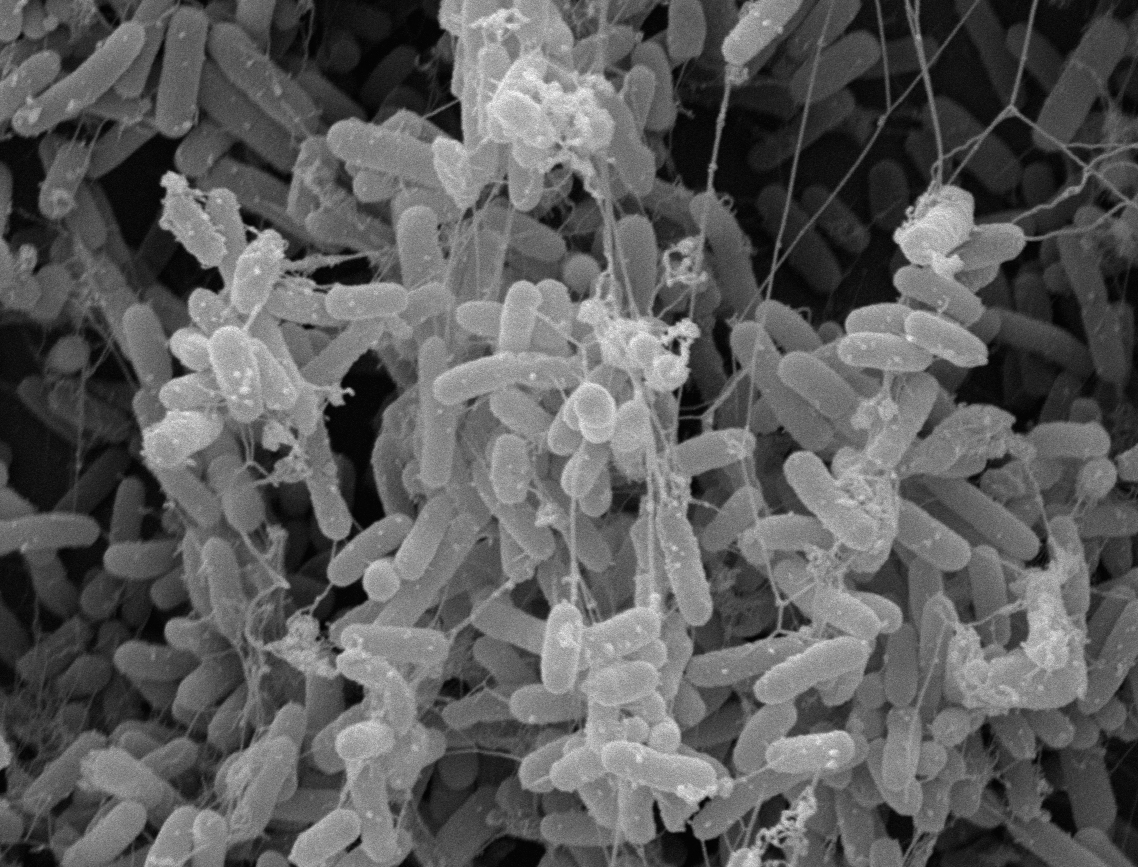
\includegraphics[width=.35\textwidth]{./20170411_environ_figs/biofilm.jpeg}
};
\end{tikzpicture}
\end{frame}


% \begin{frame}[label={sec:org569e615}]{A Brief History of Soil-persistent E. coli}
% \newcommand\ytl[2]{
% \parbox[b]{4em}{\hfill{\color{cyan}\bfseries\sffamily #1}~$\cdots\cdots$~}\makebox[0pt][c]{$\bullet$}\vrule\quad \parbox[c]{24em}{\vspace{7pt}\color{red!40!black!80}\raggedright\sffamily #2\\[7pt]}\\[-3pt]}

% \begin{table}{\small
% % \caption{A Brief Literature Review}
%  \vskip -5mm
%   \centering
%   \begin{minipage}[t]{\linewidth}
%     \color{gray}
%     \rule{\linewidth}{1pt}
%     \ytl{1886}{Escherich: Discovery of \textit{E. coli}}
%     \ytl{1948}{Bardsley: Soil may act as reservoir for \textit{E. coli}}
%     \ytl{1963}{W. and J. Boyd: Cold persistence observed }
%     %\ytl{1967}{Klein, et al: Die-off related to metabolism rates}
%     \ytl{1972}{Evans, et al: Drainage related to coliform counts} % and slurry spreading
%     \ytl{1988}{Fujioka and Shizumura: Alternative indicators suggested }
%     %\ytl{1992}{Tsai, et al: PCR detection of from soil}
%     \ytl{1997}{Texier, et al: Stable populations exist in alpine grasslands}
%     %\ytl{1998}{Byappanahalli and Fujioka: Soil extracts as growth media}
%     \ytl{2003}{Byappanahalli, et al: Soil persistence is widespread }
%     \ytl{2010}{Brennan, et al: Persistence in maritime temperate soils}
%     \bigskip
%     \rule{\linewidth}{1pt}%
%   \end{minipage}%
% } %\small
% \end{table}
% \end{frame}

\begin{frame}[label={sec:orge334fb6}]{Research Questions}
\begin{block}{Genomic Context}
\begin{itemize}
\item Are soil-persistent \emph{E. coli} related?
\item Do soil-persistent \emph{E. coli} possess certain traits?
\end{itemize}
\end{block}
\begin{block}{Virulence}
\begin{itemize}
\item Are soil-persistent strains pathogenic?
\end{itemize}
\end{block}
\end{frame}

\begin{frame}[label={sec:org0836042}]{Experimental Design: Background}
Ryan and Fanning: Effects of N and slurry on soils
\begin{itemize}
\item Isolate and protect grassland soil columns
\item Apply treatment, test leachate
\item Last application of slurry in 1998
\end{itemize}
Brennan, et al: Pathogen survival and transport in soils
\begin{itemize}
\item Two conditions: Cattle slurry and  control
\item Compare coliform counts in leachate
\end{itemize}
\end{frame}

\begin{frame}[label={sec:org06ae09a}]{Experimental Design: Current}
\begin{itemize}
\item Collect leachate from control lysimeters
\item Enrich for \emph{E. coli}
\item Purify, sequence genomes
\item Compare genomics of soil strains to wider \emph{E. coli} pangenome
\end{itemize}
\end{frame}

\begin{frame}[label={sec:org9b51ff3}]{Soil Samples}
\begin{figure}[htbp]
\centering
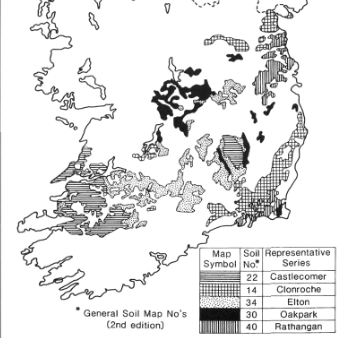
\includegraphics[width=.55\textwidth]{./lys_photos/RyanFanning1.png}
\caption{\label{fig:org7a831f6}
Lysimeter}
\end{figure}
\textsuperscript{\ref{org978fd48}}
\end{frame}

\begin{frame}[label={sec:orge15f88d}]{Lysimeters}
\begin{figure}[htbp]
\centering
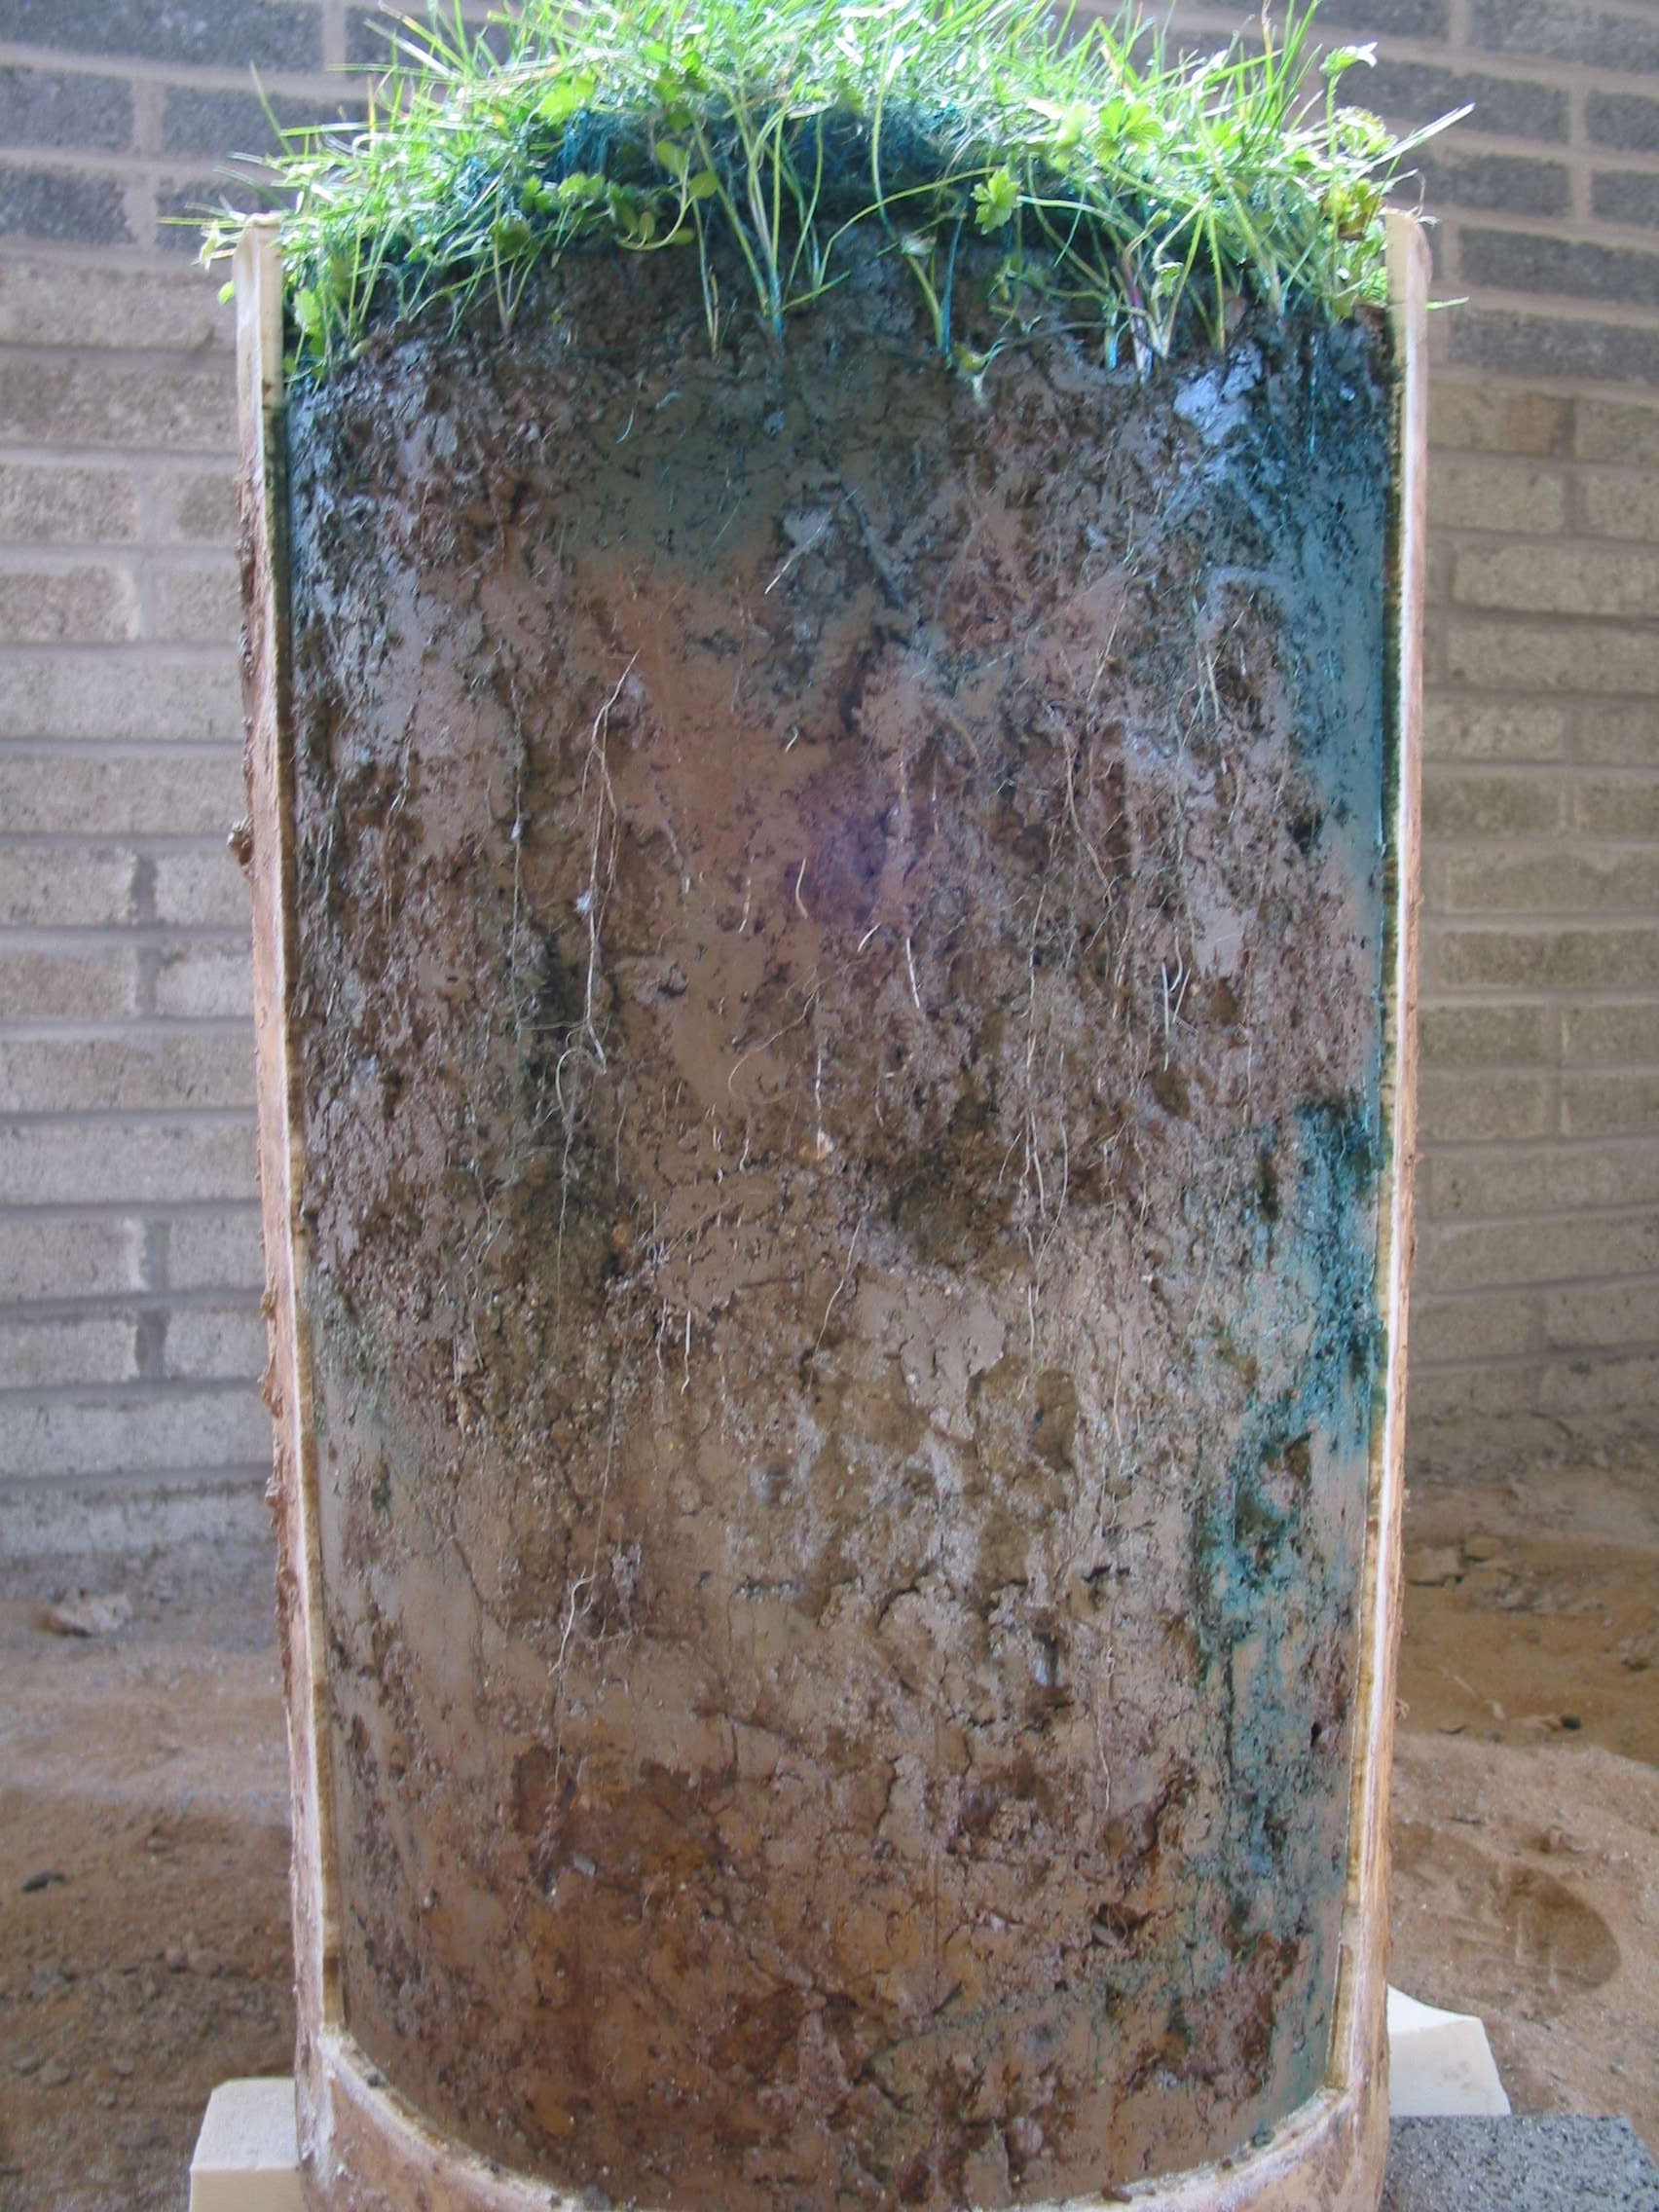
\includegraphics[width=6cm]{./lys_photos/rath2.jpg}
\caption{\label{fig:org3d3da45}
Lysimeter}
\end{figure}
\end{frame}

\begin{frame}[label={sec:org55a628a}]{Lysimeters}
\begin{figure}[htbp]
\centering
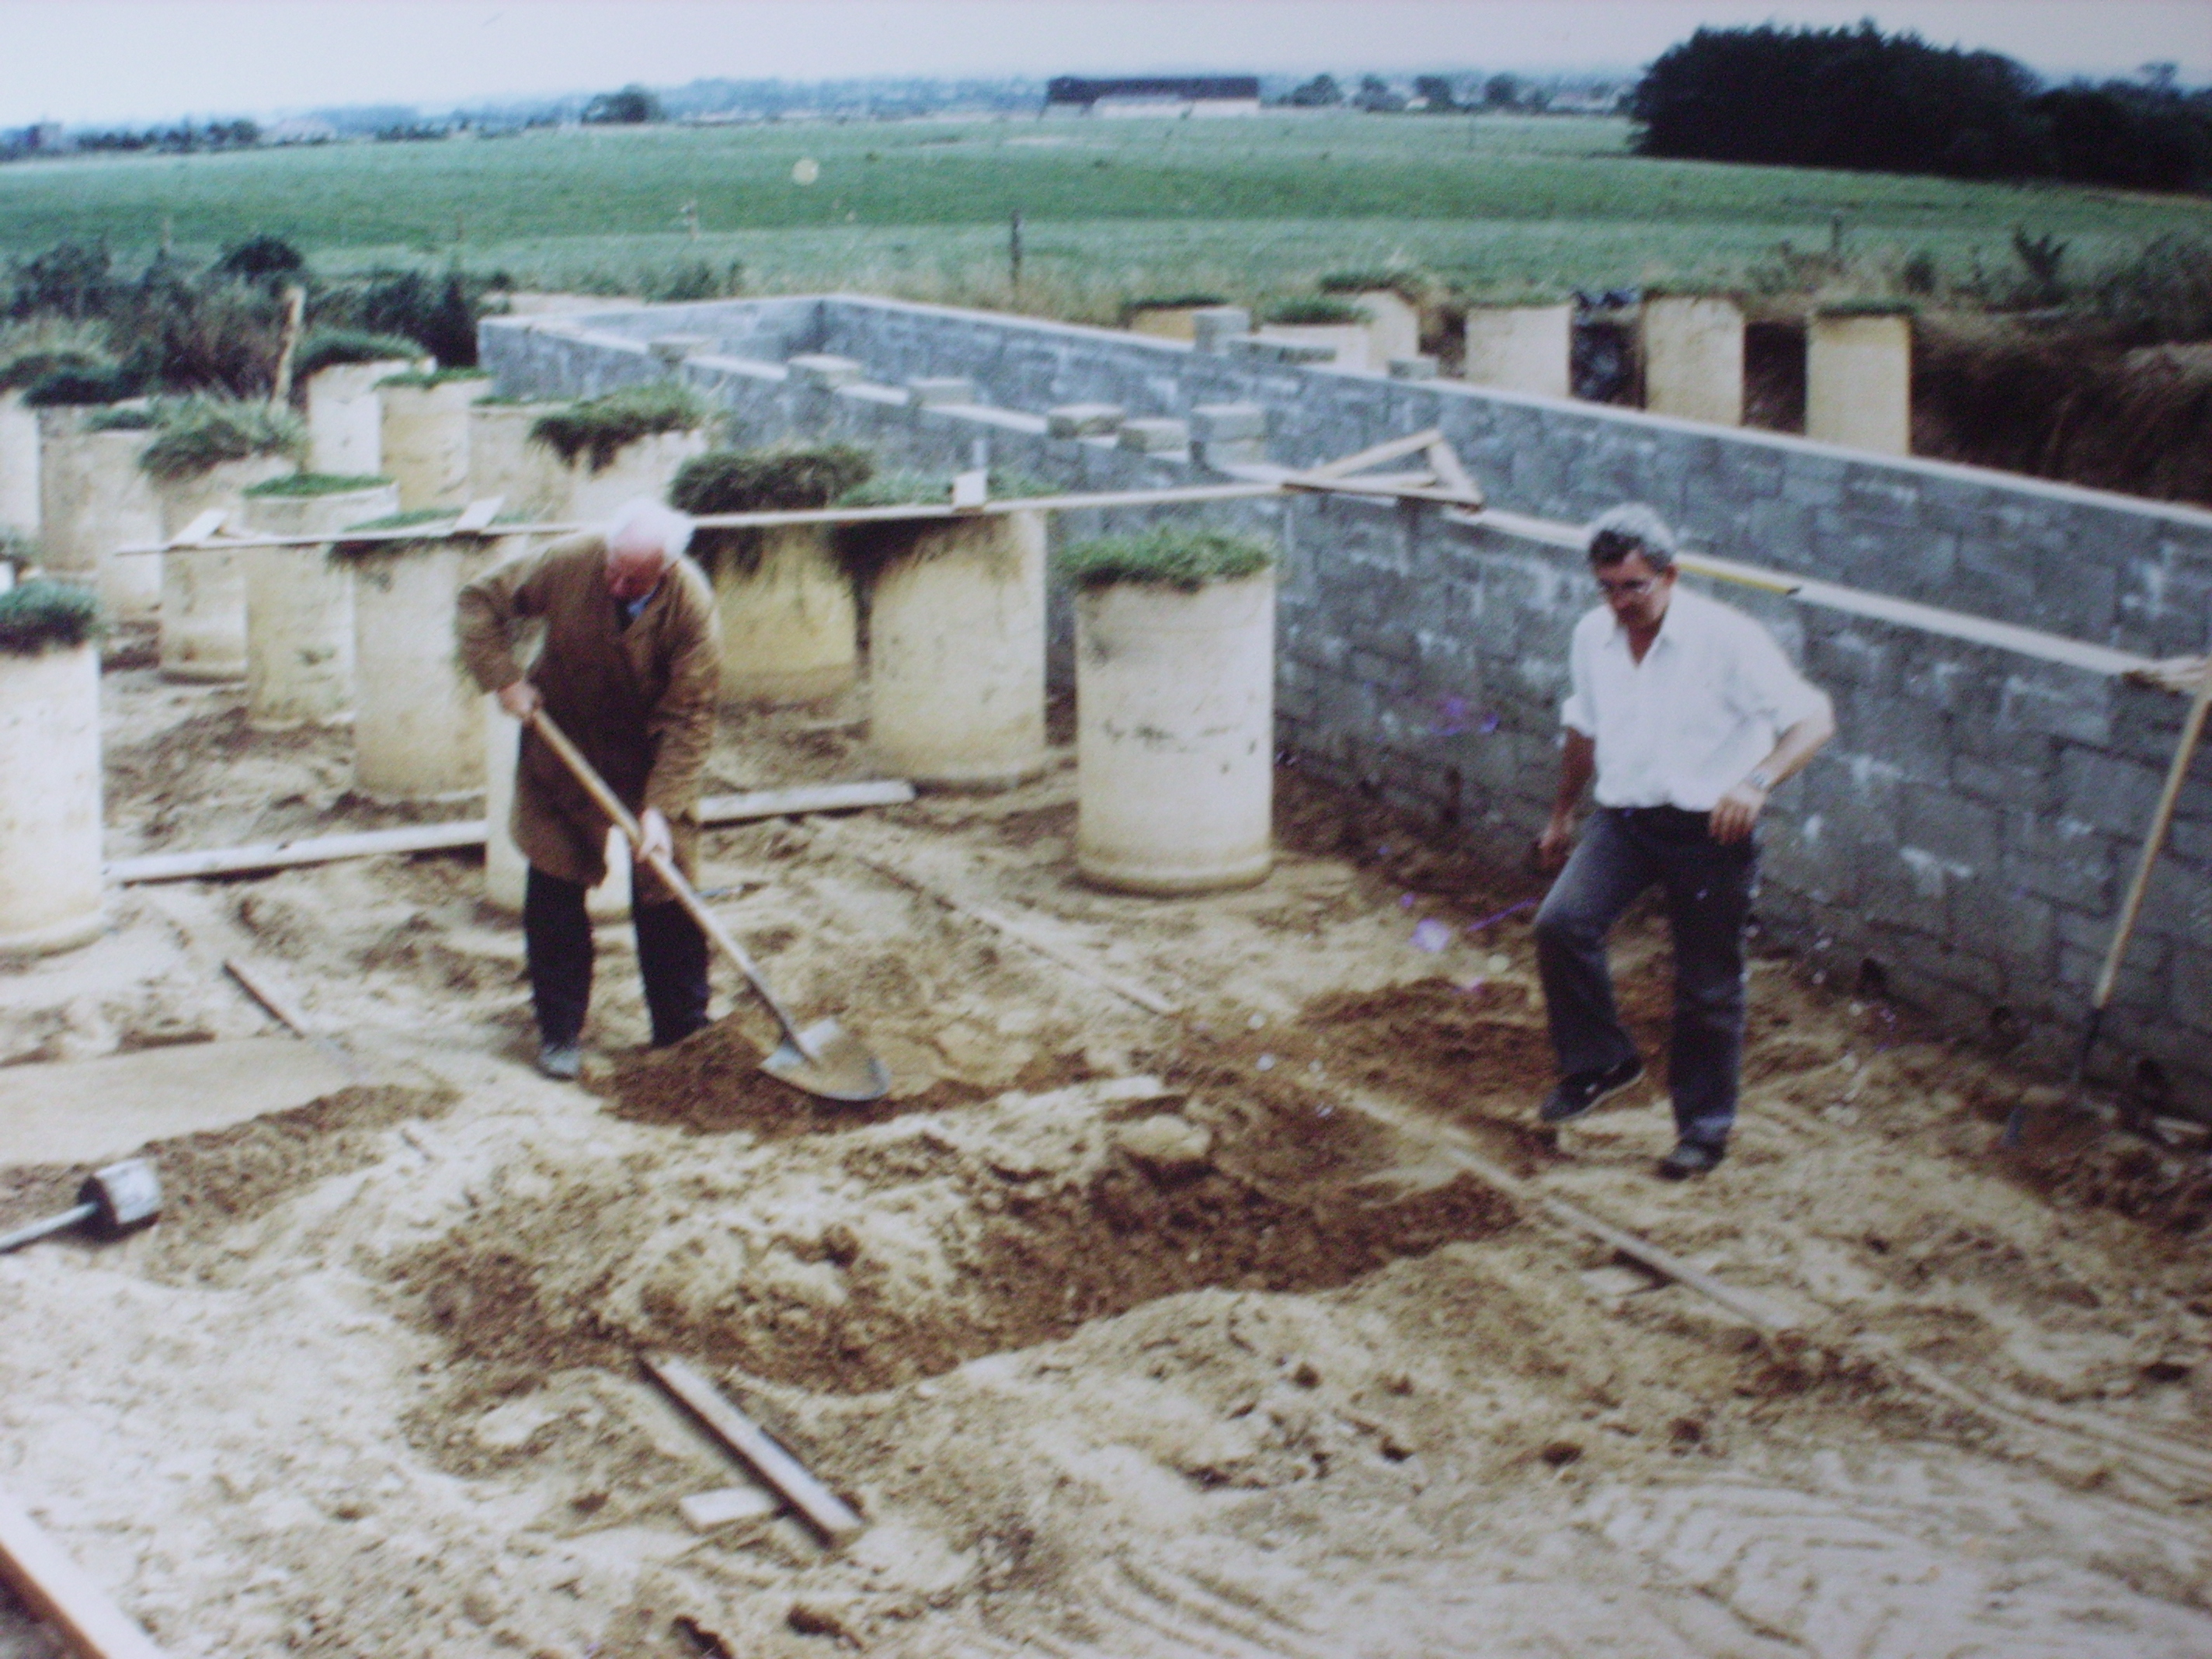
\includegraphics[width=10cm]{./lys_photos/IMGP0225.JPG}
\caption{\label{fig:orgc405371}
Lysimeter}
\end{figure}
\end{frame}

\begin{frame}[label={sec:org6eb7162}]{Lysimeters}
\begin{figure}[htbp]
\centering
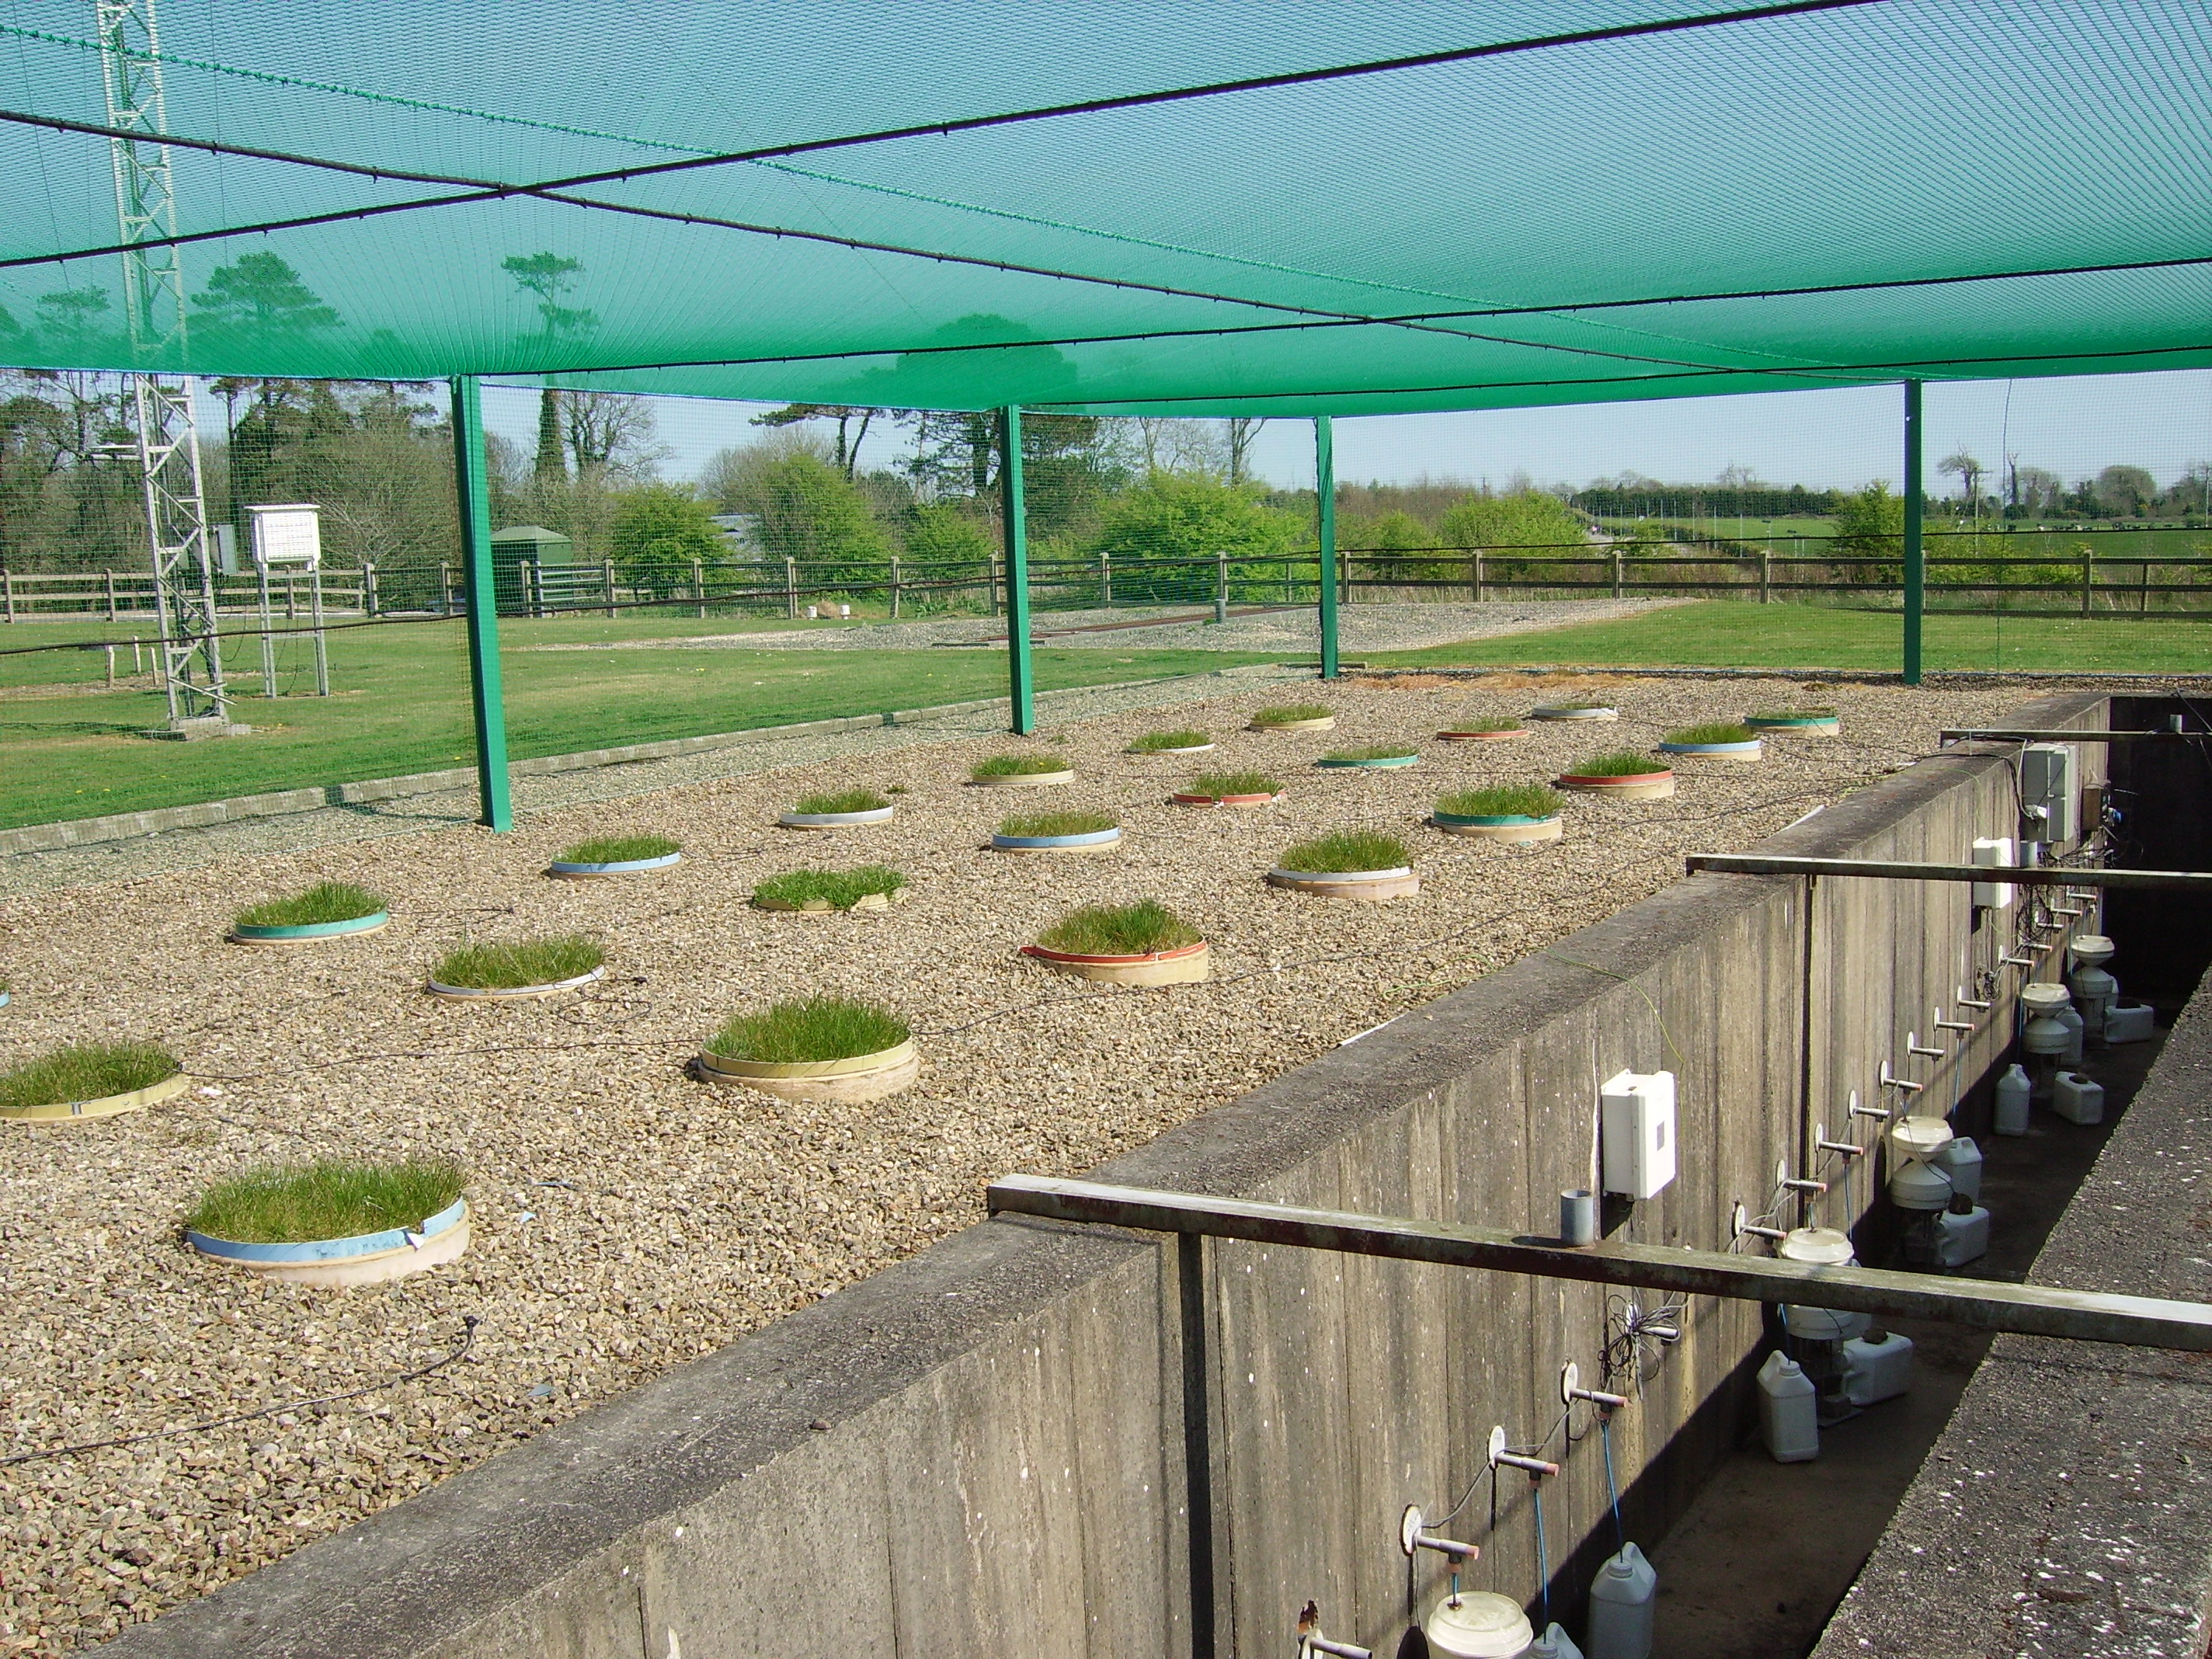
\includegraphics[width=10cm]{./lys_photos/IMGP0305.JPG}
\caption{\label{fig:org20befe1}
Lysimeter}
\end{figure}
\end{frame}

\begin{frame}[label={sec:org47ec813}]{Lysimeters}
\begin{figure}[htbp]
\centering
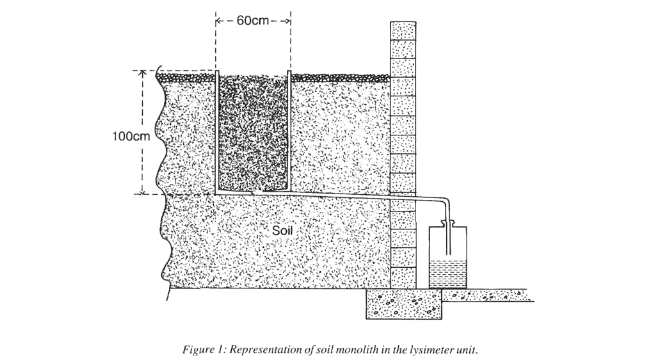
\includegraphics[width=\textwidth]{./lys_photos/RyanFanning2.png}
\caption{\label{fig:org2165260}
Lysimeter}
\end{figure}
\end{frame}



\begin{frame}[label={sec:orge1553c3}]{Workflow}
\begin{figure}[htbp]
\centering
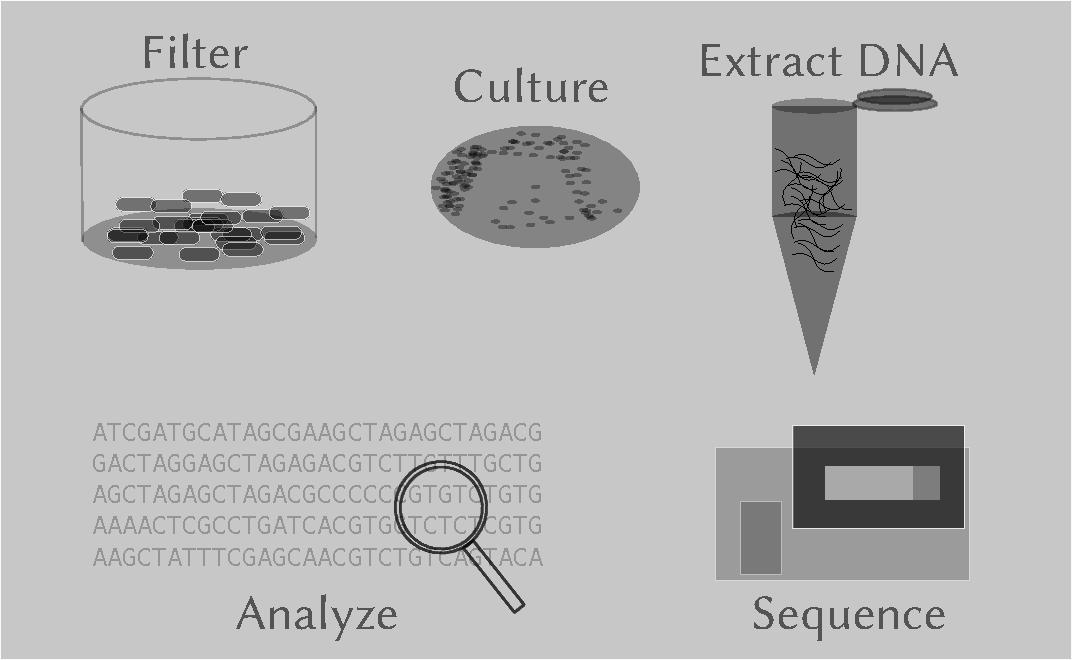
\includegraphics[width=.86\textwidth]{./frequentFigs/workflow_v1.pdf}
\caption{\label{fig:org1844168}
workflow}
\end{figure}
\end{frame}

\begin{frame}[label={sec:orgce6a1aa}]{Genomic Context}
\begin{itemize}
\item 202 isolates sequenced
\item 149 true \emph{E. coli} passed QC
\item All Clermont phylotypes represented
\end{itemize}
\begin{itemize}
\item Diverse phenotypes
\begin{itemize}
\item curli
\item metabolism
\item biofilm
\item growth rates
\end{itemize}
\end{itemize}
\begin{tikzpicture}[remember picture,overlay]
    \node[xshift=-3.5cm,yshift=-4.5cm] at (current page.north east) {
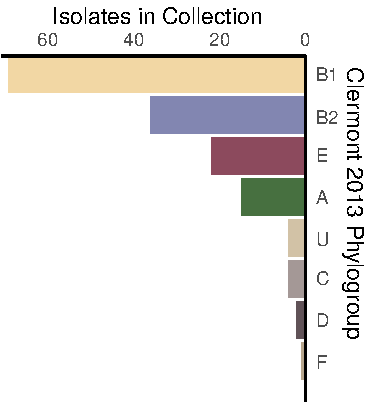
\includegraphics[width=.3\textwidth]{./2018-03-11_dc_figs/Phylogroups.pdf}
};
\end{tikzpicture}
\end{frame}

\begin{frame}[label={sec:orge91937f}]{Genomic Context}
\begin{tikzpicture}[remember picture,overlay]
    \node[xshift=-8cm,yshift=-4.8cm] (fig) at (current page.north east) {
\includegraphics[width=.55\textwidth]{./2018-03-11_dc_figs/ANIm_percentage_identity_edited.pdf}
};
\end{tikzpicture}
\end{frame}

\begin{frame}[label={sec:orgdf20357}]{Pangenome of \emph{E. coli}}
Soil-persistent E. coli (149)

Comparison E. Coli (1300)
\end{frame}

\begin{frame}[label={sec:orga25860d}]{}
  \includegraphics[height=\textheight]{./2018-03-11_dc_figs/2017-08-21reduced_snptree.pdf}
\end{frame}

\begin{frame}[label={sec:orga25860d}]{}
  \includegraphics[width=10cm]{./2018-03-11_dc_figs/2017-08-22reduced_snptree_clade_C_node_1882.pdf}
\end{frame}


\begin{frame}[label={sec:orga25860d}]{}
  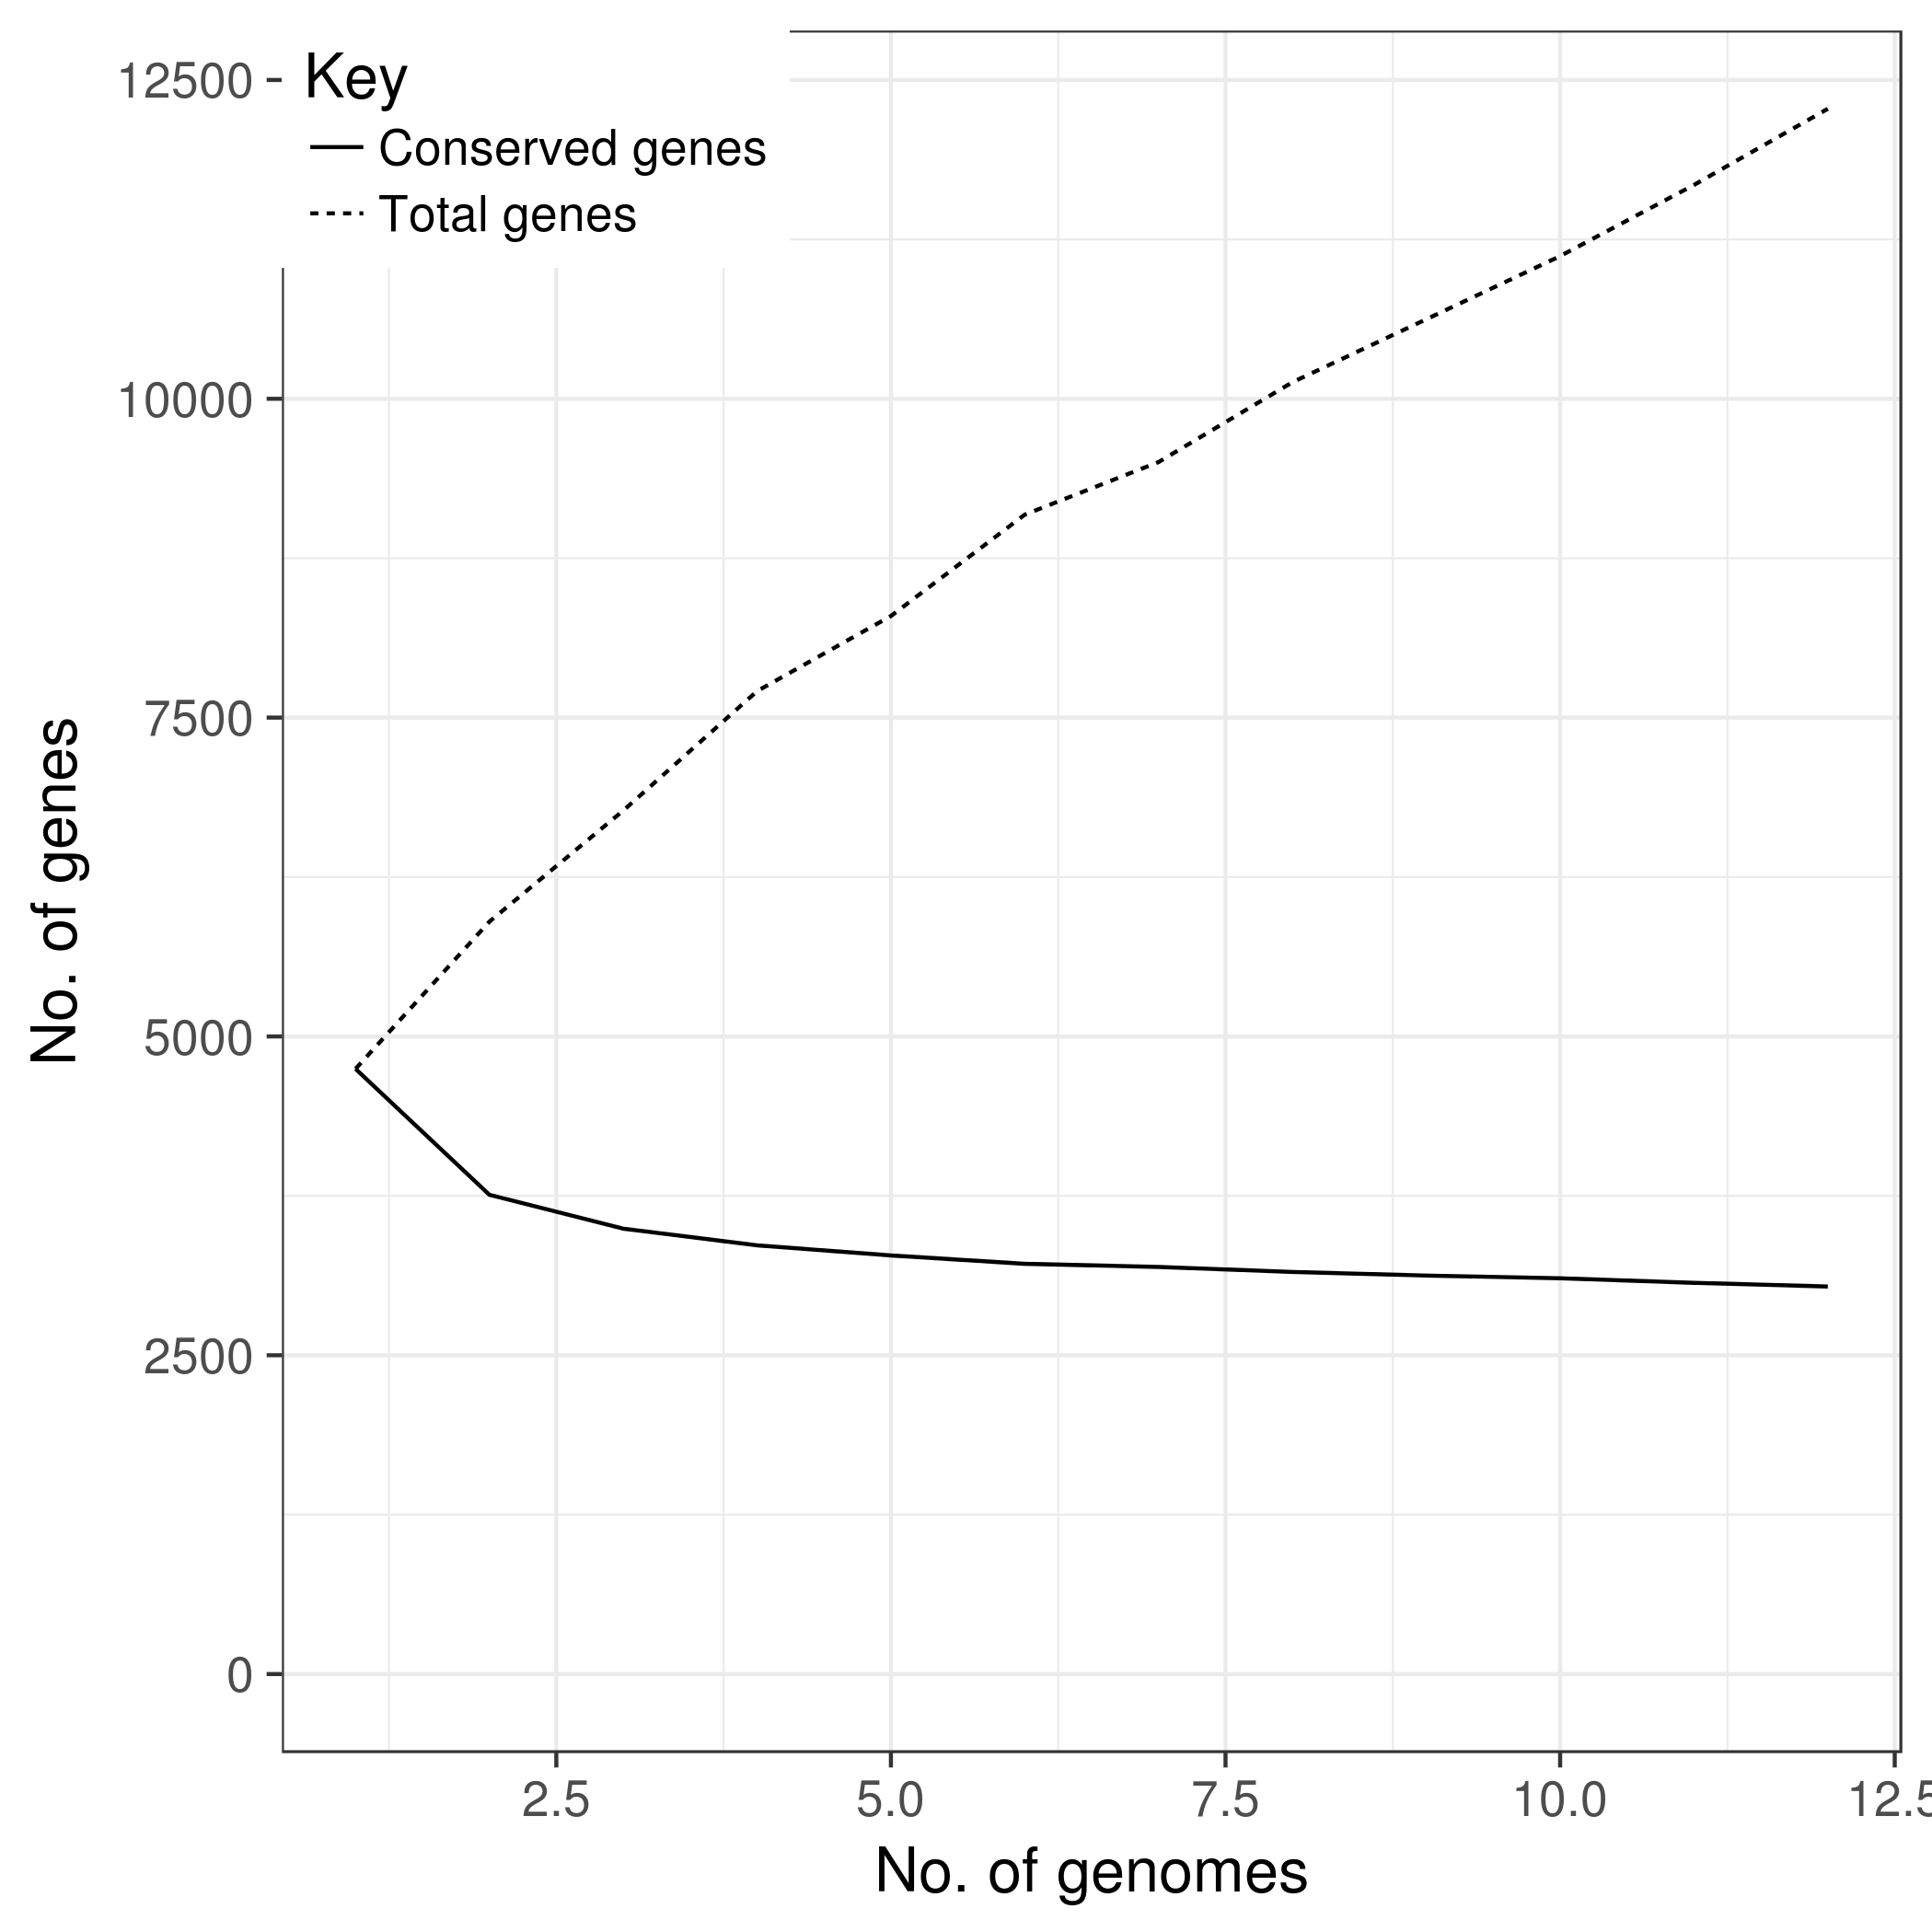
\includegraphics[height=\textheight]{./2018-03-11_dc_figs/conserved_vs_total_genes.png}
\end{frame}

\begin{frame}[label={sec:orga25860d}]{}
  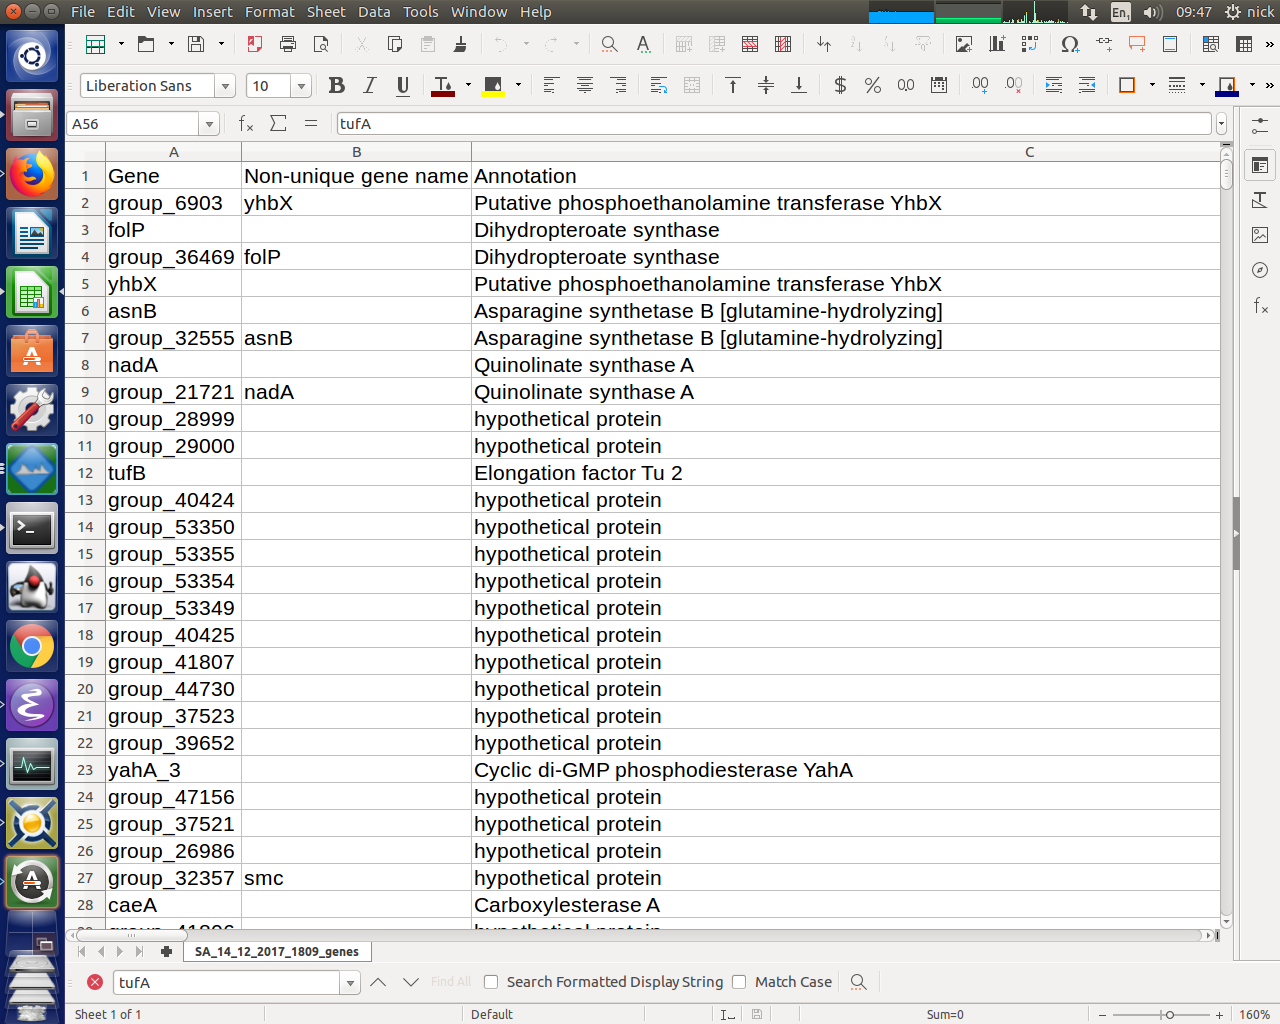
\includegraphics[width=10cm]{./2018-03-11_dc_figs/multiple.png}
\end{frame}

\begin{frame}[label={sec:orga25860d}]{}
  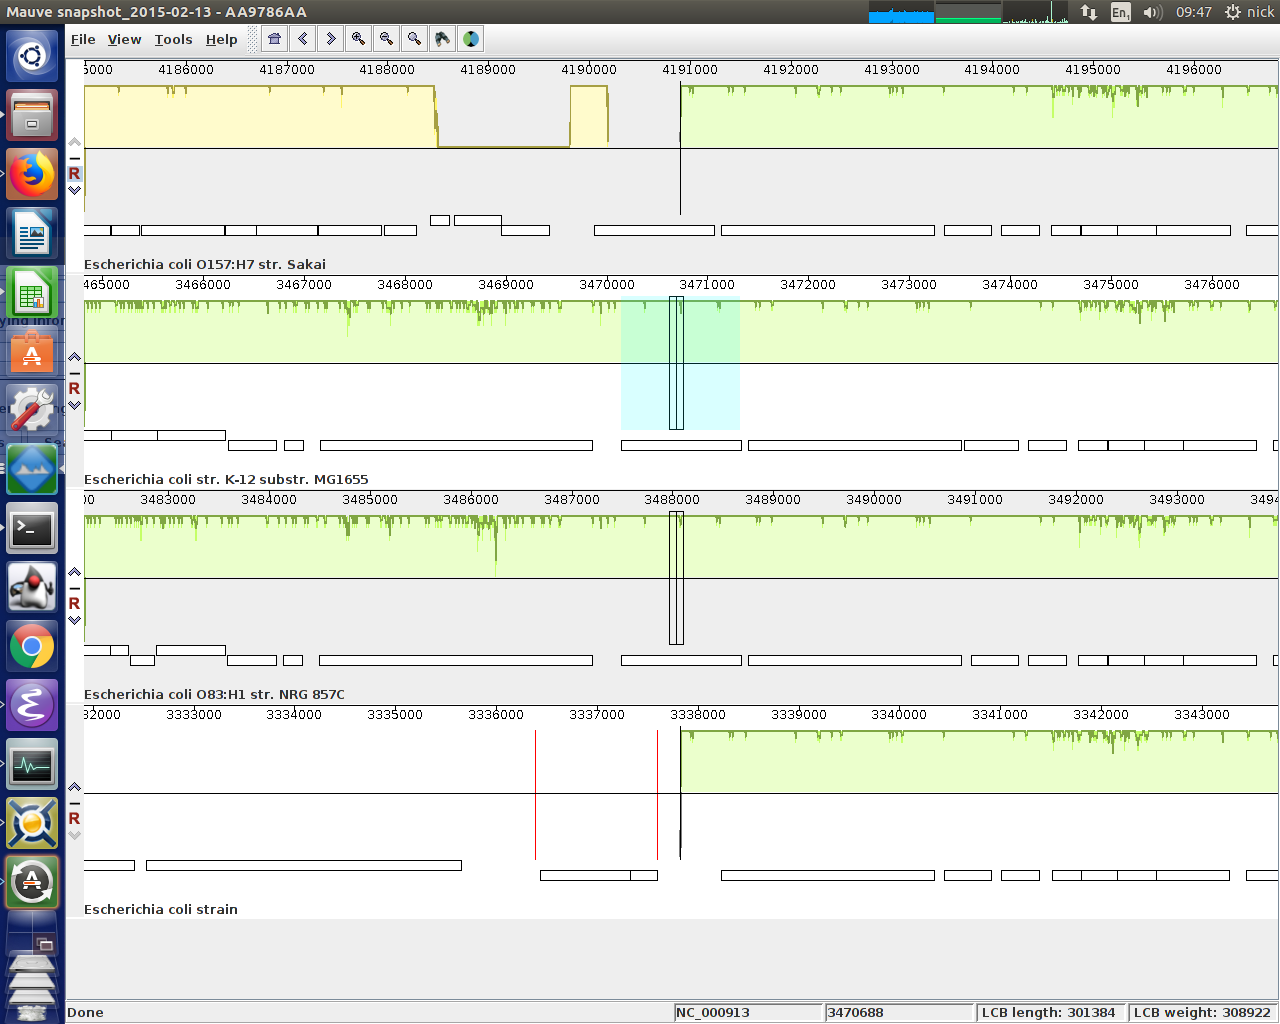
\includegraphics[width=10cm]{./2018-03-11_dc_figs/tufA.png}
\end{frame}


% \begin{frame}[label={sec:org86efded}]{Virulence}
% \begin{itemize}
% \item Search literature for genes implicated in virulence
% \item Select representative sequences for \textasciitilde{}50 virulence factors
% \item Use reciprocal translated blast to find occurrences
% \item Filter results, visualize
% \end{itemize}
% \end{frame}

% \begin{frame}[label={sec:orge53e9c0}]{Virulence Results}
% \hspace{1.5cm}\begin{tikzpicture}[spy using outlines={red,magnification=4, size=3.5cm,connect spies}]
%     \node[anchor=south west,inner sep=0] (image) at (0,0) {
%    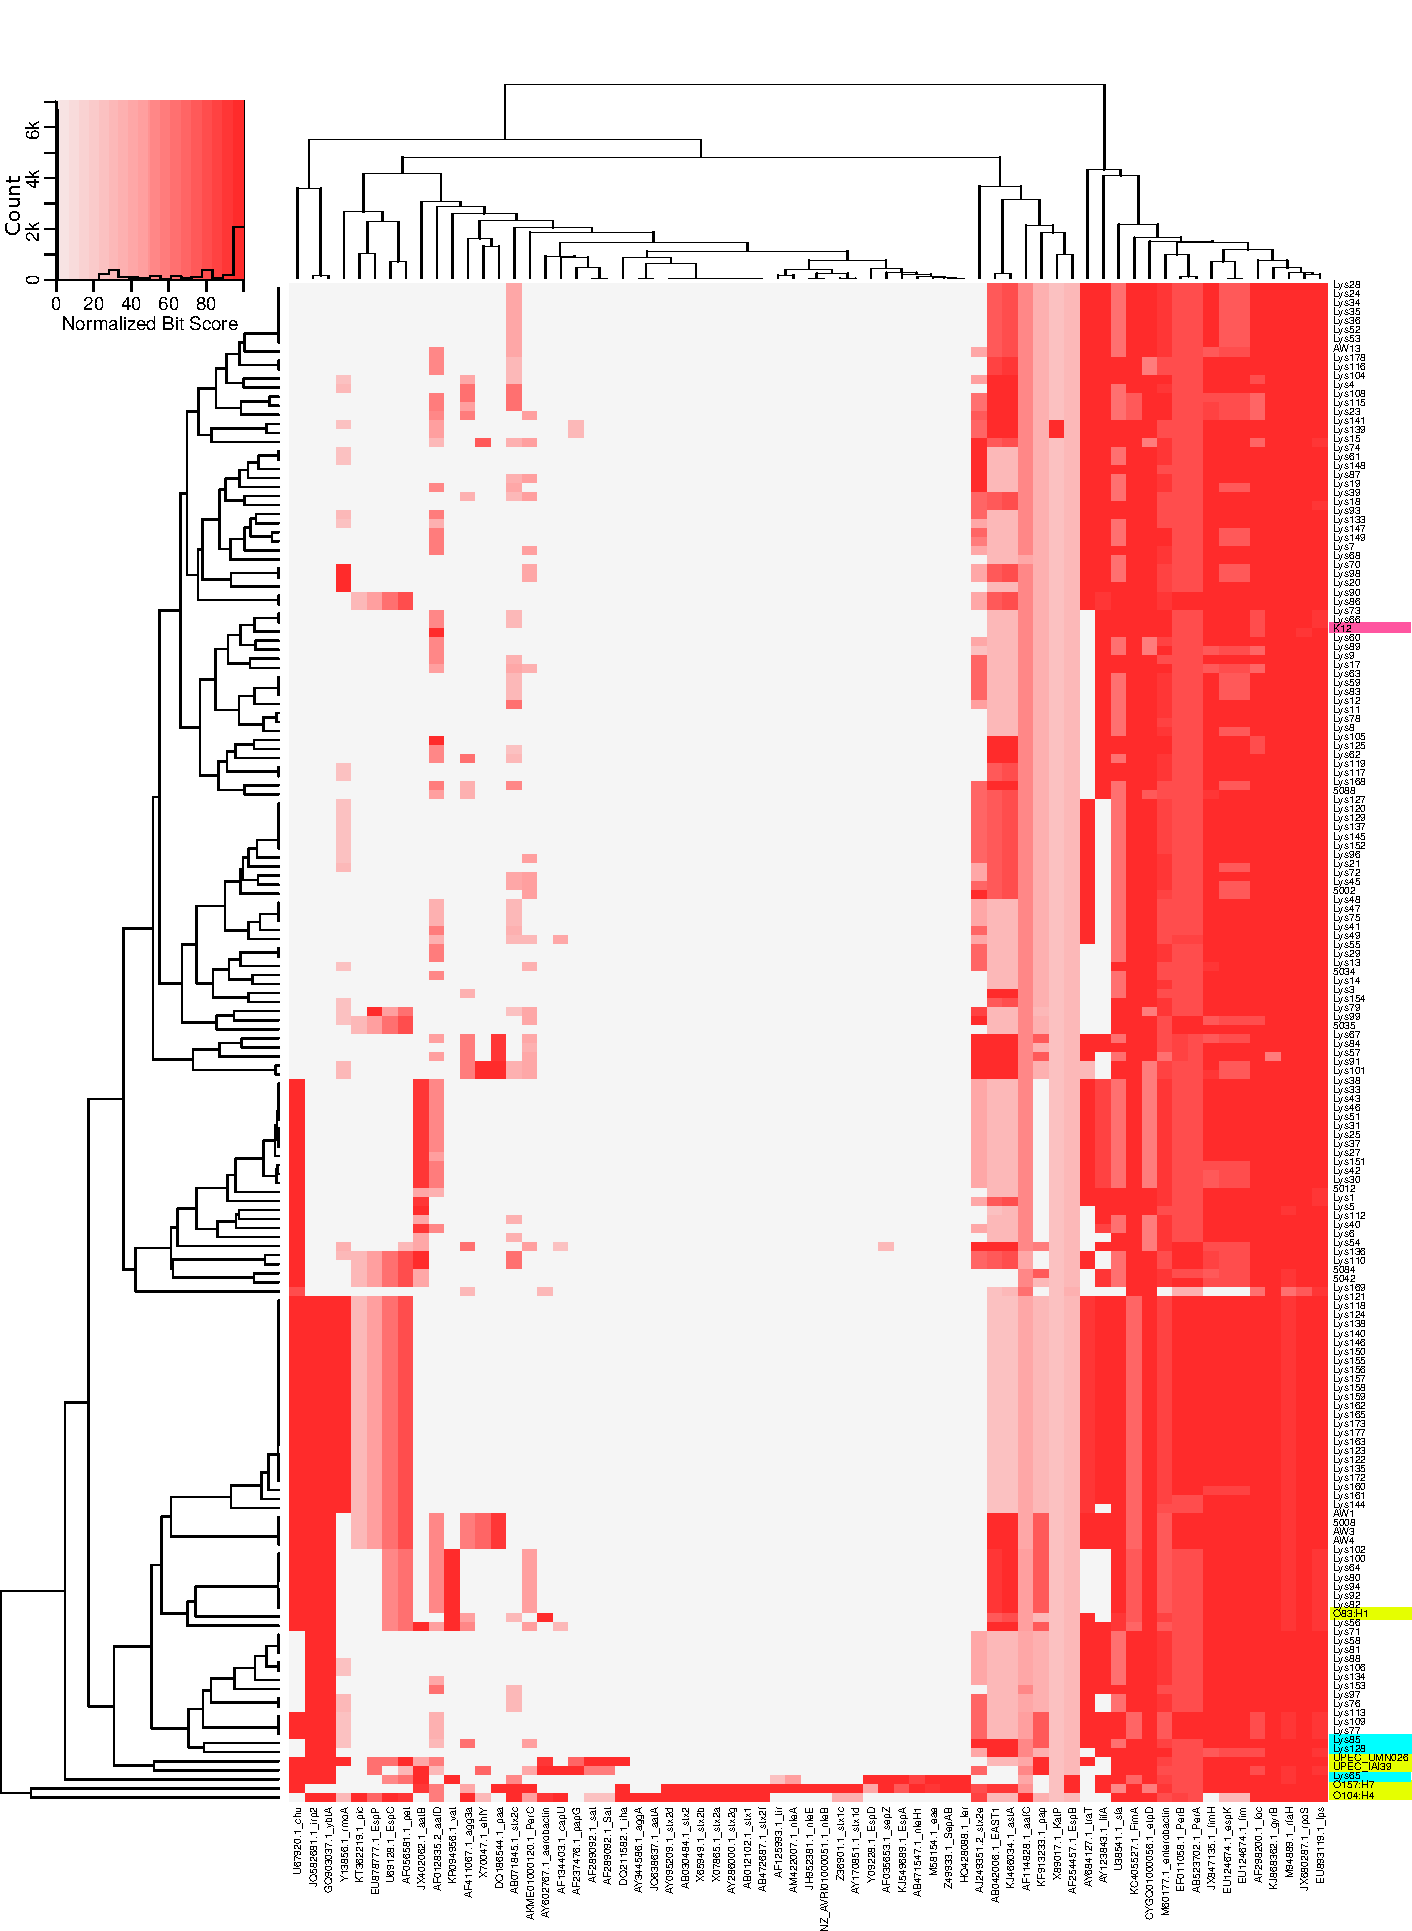
\includegraphics[width=5cm]{./2018-03-11_dc_figs/blastheatmap.pdf}};
%    \spy on ($0.9*(image.south east)+0.19*(image.west)$) in node at ([xshift=-2cm]image.west);
% \end{tikzpicture}
% \end{frame}




\begin{frame}[label={sec:orga1ea581}]{Conclusions about Soil-persistent \emph{E. coli}}
\begin{itemize}
\item Represent diverse lineages
\item Posess a range of virulence genes
\item May pose a human health threat
\item Complicate use of \emph{E. coli} as contamination indicator
\end{itemize}
\end{frame}



\begin{frame}[label={sec:orgbbb97da}]{Current Issues}
\begin{itemize}
\item Screening missassembled genes from pangenome analysis
\item Explore genomes for markers associated with soil isolates
\item Explore trends potentially relating function to environmental factors
\end{itemize}
\end{frame}


\begin{frame}[label={sec:orgb172077}]{Sources}
\tiny
\begin{description}
\item[{Bardsley, D.}] "A study of coliform organisms in the Melbourne water supply and in animal faeces, with observations on their longevity in faeces and in soil." \uline{The Journal of Hygiene}, 46(3), 269–79. 1948
\item[{Brennan, et al.}] "Characterization of environmentally persistent escherichia coli isolates leached from an irish soil." \uline{Applied and Environmental Microbiology}, 76(7), 2175–2180. 1996
\item[{Boyd, W and J.}] "Viability of Coliform Bacteria In Antarctic Soil." \uline{Journal of Bacteriology}, 84. 1963
\item[{Byappanahalli, et al.}] "Population structure, persistence, and seasonality of autochthonous Escherichia coli in temperate, coastal forest soil from a Great Lakes watershed". \uline{Environmental Microbiology}, 8(3), 504–513. 2006
\item[{Kirk, et al}] "World Health Organization Estimates of the Global and Regional Disease Burden of 22 Foodborne Bacterial, Protozoal, and Viral Diseases, 2010: A Data Synthesis." \uline{Plos Medicine} 2015
\item[{Pruess, B.}] \emph{E. coli} image. \uline{NDSU Agriculture Comm.} April 29, 2011
\item[{Ryan and Fanning}] "Effects of fertiliser N and slurry on nitrate leaching - lysimeter studies on 5 soils." \uline{Irish Geography}  29(2) 1996
\end{description}
\end{frame}


\begin{frame}[label={sec:org92bea95}]{Acknowledgments}
\small
  \begin{columns}[onlytextwidth]
    \column{0.5\textwidth}
    
\includegraphics[height=1cm]{2018-03-11_dc_figs/NUI_Galway_BrandMark_A_K-eps-converted-to.pdf}\\
     NUIG Microbiology
      \begin{itemize}
        \item Dr. Fiona Brennan
        \item Dr. Florence Abram
%        \item Matthias Waibel
%        \item Stephen Nolan
%        \item Camilla Thorn
      \end{itemize}

    \column{0.5\textwidth}
    \vskip .25em
    
\includegraphics[height=1cm]{2018-03-11_dc_figs/trimmed_jhi.png}\\
      James Hutton Institute, Dundee
      \begin{itemize}
        \item Dr. Leighton Pritchard
        \item Dr. Ashleigh Holmes
      \end{itemize}
\vskip 1cm
       \huge Questions?
  \end{columns}
\end{frame}
\end{document}